Since the production cross-section for Drell-Yan is several orders of magnitude 
higher than the $H \to ZZ$ signal, the Drell-Yan background poses a significant 
challenge. To the leading order, the Drell-Yan process does not contain \met\,  
and therefore its contribution is signficantly reduced by a tight \met selection. 
The residual Drell-Yan contribution in the signal region 
is mainly due to events with fake \met either due to energy mismeasurement of  
the hadronic recoil or momentum mismeasurement of the selected leptons. 
The contribution of events with fake \met due to the lepton momentum mismeasurement 
is expected to be small since we select events within a fairly tight (within $15$ GeV) window 
around the $Z$ boson pole mass. The background due to mismeasurement of the hadronic
recoil is the main source of Drell-Yan events contributing to the selected signal region.

The estimation of residual Drell-Yan background in the signal region depends highly 
our understanding of the \met tails which is sensitive to many factors such as 
the jet energy corrections, the number of pileup interactions, and energy from out of time
contributions. These effects are difficult to model precisely in the simulation.
Therfore we employ a data-driven method to estimate the \met distribution for the 
Drell-Yan background. For events without natural \met\, under the assumption that 
the fake \met is only resulting from mismeasurement of the hadronic recoil, we can use
$\gamma$+jets events as a control sample to predict the \met distribution in $Z$+jets
background events. If parameterized correctly in an observable that is highly correlated 
with the source of fake \met, one expects $\gamma$+jets events to provide an accurate
model of the \met distribution for $Z$+jets events, provided that the photon
is well measured and does not contribute to the \met.

\subsubsection{Photon Selection and Reweighting Procedure}
The photon data sample is selected by requiring one and only one photon passing reaonsably tight
identification and isolation requirements, summarized in Table \ref{tab:PhotonSelection} below 
\cite{MITHggNote}. 
An electron veto is imposed on the photon, requiring that no GSF electron which does not match to 
one leg of a well reconstructed conversion is sharing the same supercluster as the photon
candidate. This is intended to reduce contributions from W bosons decaying to electrons, misidentified
as photons. To reduce contamination from $W$+$\gamma$ events, we veto any events with one or 
more well identified leptons.


\begin{table}[!ht]
\begin{center}
\begin{tabular}{|c|c|} 
\hline
Cut           & Requirement                                                                           \\
\hline
$\eta$        & $|\eta| < 1.4442$                                                                     \\ 
\hline
H/E           & H/E $< 0.05$                                                                          \\
\hline
Electron Veto & Photon is rejected if it shares the supercluster with an electron that does not       \\
              & match to one leg of a conversion with $\mathrm{L}_{\mathrm{xy}} < 2.0$, fit           \\
              & probability  $> 10^{-6}$, and no hits behind the fitted vertex                        \\
\hline
\hline
\multicolumn{2}{|c|}{Conversion ID (if matched to a conversion with $\mathrm{L}_{\mathrm{xy}} < 2.0$,}\\
\multicolumn{2}{|c|}{fit probability $> 10^{-6}$, and at most one hit before the fitted vertex on }   \\
\multicolumn{2}{|c|}{either of the tracks forming the conversion) }                                   \\
\hline
E/P            & E/P $< 2.0 $                                                                         \\
%$\Delta\eta$  & $|\Delta\eta| < 0.01 for Endcap only$ \\
%$\Delta\phi$  & $|\Delta\phi| < 0.01 for Endcap only$ \\
\hline
\hline
\multicolumn{2}{|c|}{Isolation}                                                                       \\
\hline
EcalIso       & EcalIso $ - \rho\times \mathrm{A}_{\mathrm{eff Ecal}}$ $<  2.0 + 0.006\times p_{T}$   \\
HcalIso       & HcalIso $ - \rho\times \mathrm{A}_{\mathrm{eff Hcal}}$ $<  2.0 + 0.0025\times p_{T}$  \\
TrkIso        & TrkIso $ - \rho\times \mathrm{A}_{\mathrm{eff Trk}}$ $<  1.5 + 0.001\times p_{T}$     \\
\hline

%\hline
%SpikeKilling & \\
%\hline
%$E_{\mathrm{Max}} / E_{9}$ & $E_{\mathrm{Max}} / E_{9} > 0.95$       \\
%$\sigma_{i\eta i\eta}$     & $\sigma_{i\eta i\eta} > 0.001$          \\
%$\sigma_{i\phi i\phi}$     & $\sigma_{i\phi i\phi} > 0.001$          \\
%\hline

\hline
\end{tabular}
\caption{MC yield prediction for $H\rightarrow WW$ sample ($m_H=130$ GeV) ($\mu$-e and e-e final states). 
The electron selection is the same as in 2010 analysis and the results is scaled to 1/fb.
\label{tab:PhotonSelection}}
\end{center}
\end{table}

Since the fake \met is due to mismeasurement of the hadronic recoil, we parameterize the 
modelling of the \met distribution in the $p_{T}$ of the photon / dilepton system and 
the number of counted jets. Both variables are highly correlated with the behavior 
of the hadronic recoil. Reweighting factors are computed in bins of the number of counted jets
and the dilepton $p_{T}$ by dividing the corresponding two dimensional distributions
in the $\gamma$+jets data sample and the dilepton data sample:

\begin{eqnarray}
  w(p_{T},\mathrm{njet}) = \frac{\mathrm{N}_{\gamma+\mathrm{jets}}(p_{T},\mathrm{njet})}{\mathrm{N}_{\mathrm{Z+jets}}(p_{T},\mathrm{njet})}.
\end{eqnarray}

In order for these reweighting factors to be insensitive to the presence of signal or backgrounds with 
real \met, we build these weight factors on a $\gamma$+jets and $Z$+jets sample imposing an anti-selection
on the minimum of the \met and the track \met at below $50$ GeV. For the $Z$+jets sample, 
the full $H \to ZZ$ preselection is imposed, 
including the top veto and the third lepton veto.

Finally, to model the \met distribution for the final selection we select $\gamma$+jets events
as above, imposing the preselection requirement that the photon $p_{T}$ is greater than $40$GeV,
and associate the corresponding weight factor $w(p_{T},\mathrm{njet})$ to each such event. To build
the track \met in the $\gamma$+jets events, we must consistently account for the momentum of
the photon since we intend it to model the dilepton system which would be included in the 
track \met in $Z$+jets events. To mitigate cases of inconsistencies between the particle flow 
photon reconstruction and the standard photon reconstruction, particularly for converted photons,
we do not include any charged particle flow candidates inside the ($\Delta$R $<0.4$) isolation cone 
of the photon in the track \met sum.
To model the transverse mass distribution, we draw a random number from a pre-determined dilepton
mass distribution and build the $m_{T}$ observable as in Eqn \ref{}. The dilepton mass distribution
is constructed from data imposing all preselection cuts except the \met requirement.

\subsubsection{Monte Carlo Closure Test}

In order to verify that the procedure models the $Z$+jet background well, we test it
in $\gamma$+jets and $Z$+jets Monte Carlo simulation. The reweighting factors are 
built from the simulation sample according to the procedure described above and then 
applied on the $\gamma$+jets Monte Carlo sample. 

%The photon and $Z$ 
%$p_{T}$ distributions are shown in Fig \ref{fig:PhotonJetsClosureTest_Pt} to demonstrate that 
%the reweighting is carried out consistently.

%% \begin{figure}[!htbp]
%% \begin{center}
%% \subfigure[0-Jet]{\includegraphics[width=0.45\textwidth]{figures/PhotonJetsClosureTest_0Jet_Pt.pdf}}
%% \subfigure[1-Jet]{\includegraphics[width=0.45\textwidth]{figures/PhotonJetsClosureTest_1Jet_Pt.pdf}}
%% \subfigure[2-Jet]{\includegraphics[width=0.45\textwidth]{figures/PhotonJetsClosureTest_2Jet_Pt.pdf}}
%% \caption{Comparison of the dilepton $p_{T}$ and the photon $p_{T}$ before and after reweighting.}
%% \label{fig:PhotonJetsClosureTest_Pt}
%% \end{center}
%% \end{figure}


In Fig \ref{fig:PhotonJetsClosureTest_TrackMET} we show the particle flow \met distribution 
from the $\gamma$+jet sample after reweighting compared to the \met distribution from the 
$Z$+jet sample, separately in the 0-jet, 1-jet, and 2-jet bins. We observe agreement between 
the $\gamma$+jet generated prediction and the $Z$+jet simulation particle flow \met distribution. 
In Fig \ref{fig:PhotonJetsClosureTest_TrackMET} we show the analogous comparison for track \met, where 
is agreement slightly worse than for particle flow \met. Finally, in 
Fig \ref{fig:PhotonJetsClosureTest_TrackMET}, we show the comparison for the minimum of the 
track \met and the particle flow \met, which shows better agreement than the track \met alone. 

\begin{figure}[!htbp]
\begin{center}
\subfigure[0-Jet]{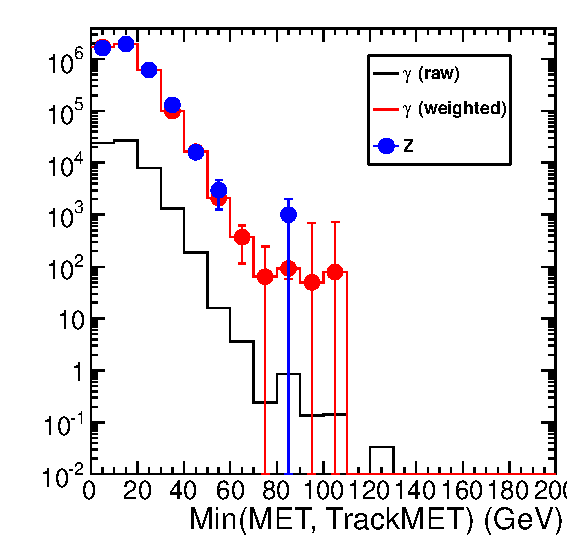
\includegraphics[width=0.3\textwidth]{figures/PhotonJetsClosureTest_0Jet_PFMET.pdf}}
\subfigure[1-Jet]{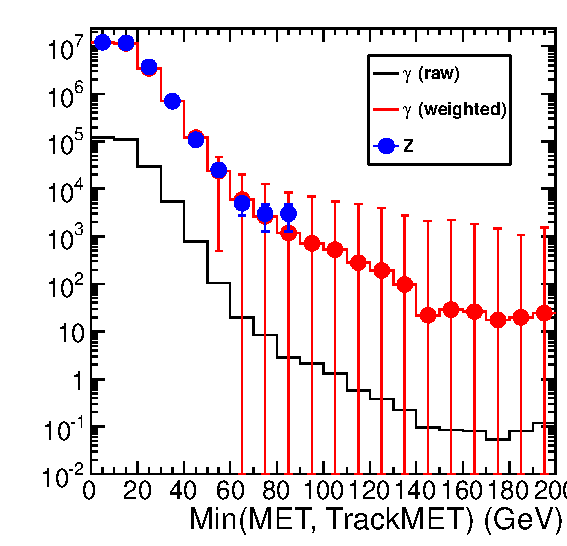
\includegraphics[width=0.3\textwidth]{figures/PhotonJetsClosureTest_1Jet_PFMET.pdf}}
\subfigure[2-Jet]{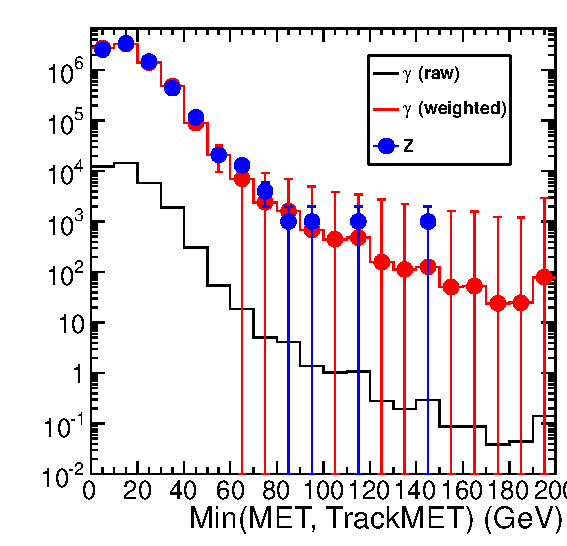
\includegraphics[width=0.3\textwidth]{figures/PhotonJetsClosureTest_2Jet_PFMET.pdf}}
\caption{Comparison of the particle flow \met prediction from the reweighted $\gamma$+jets sample
and the simulation prediction from the $Z$+jets sample.}
\label{fig:PhotonJetsClosureTest_TrackMET}
\end{center}
\end{figure}

\begin{figure}[!htbp]
\begin{center}
\subfigure[0-Jet]{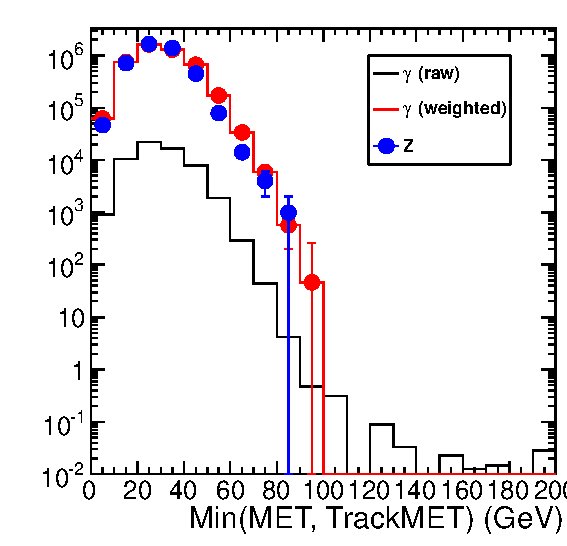
\includegraphics[width=0.3\textwidth]{figures/PhotonJetsClosureTest_0Jet_TrackMET.pdf}}
\subfigure[1-Jet]{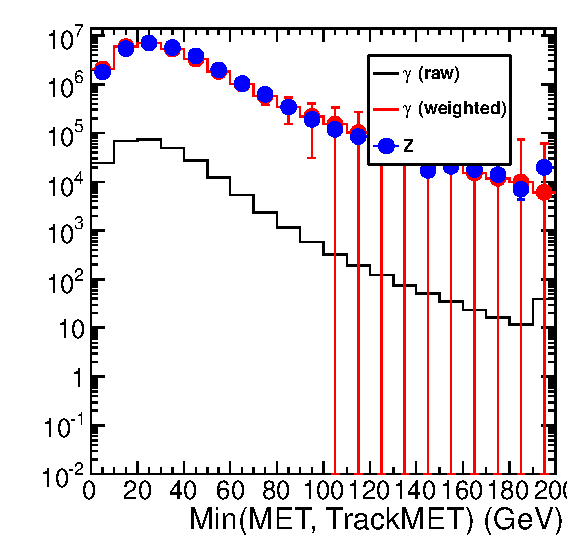
\includegraphics[width=0.3\textwidth]{figures/PhotonJetsClosureTest_1Jet_TrackMET.pdf}}
\subfigure[2-Jet]{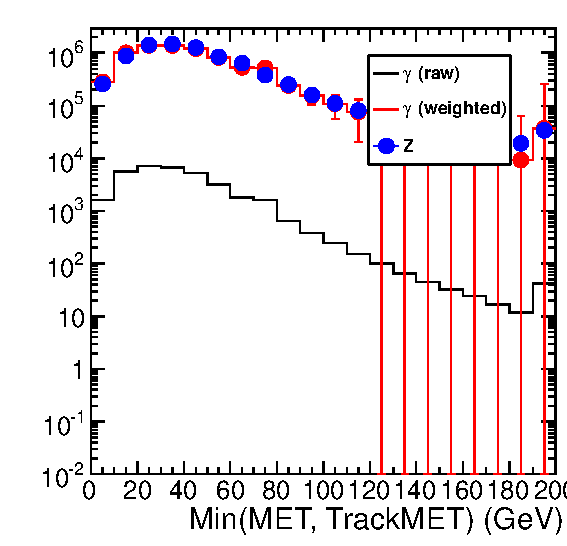
\includegraphics[width=0.3\textwidth]{figures/PhotonJetsClosureTest_2Jet_TrackMET.pdf}}
\caption{Comparison of the particle flow track \met prediction from the reweighted $\gamma$+jets sample
and the simulation prediction from the $Z$+jets sample.}
\label{fig:PhotonJetsClosureTest_TrackMET}
\end{center}
\end{figure}

\begin{figure}[!htbp]
\begin{center}
\subfigure[0-Jet]{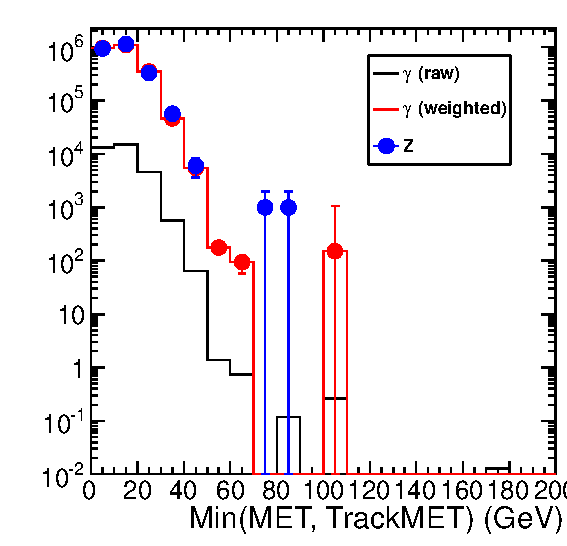
\includegraphics[width=0.3\textwidth]{figures/PhotonJetsClosureTest_0Jet_MinMET.pdf}}
\subfigure[1-Jet]{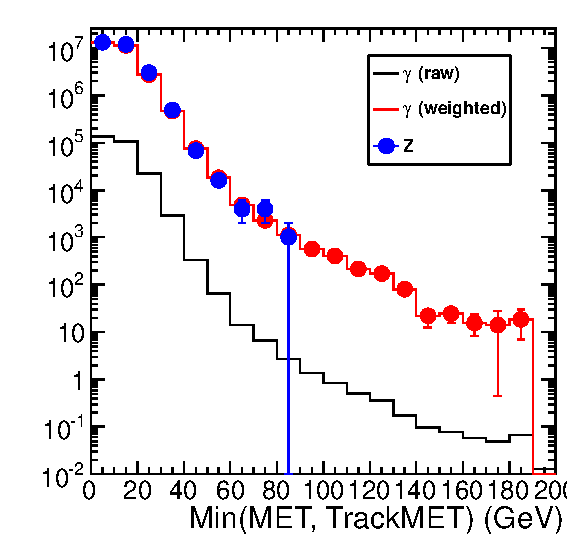
\includegraphics[width=0.3\textwidth]{figures/PhotonJetsClosureTest_1Jet_MinMET.pdf}}
\subfigure[2-Jet]{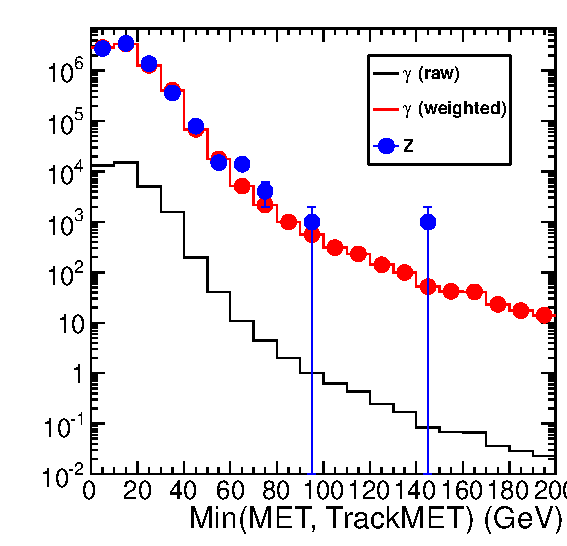
\includegraphics[width=0.3\textwidth]{figures/PhotonJetsClosureTest_2Jet_MinMET.pdf}}
\caption{Comparison of the minimum of particle flow \met and particle flow track \met prediction from
the reweighted $\gamma$+jets sample and the simulation prediction from the $Z$+jets sample.}
\label{fig:PhotonJetsClosureTest_TrackMET}
\end{center}
\end{figure}

\begin{figure}[!htbp]
\begin{center}
\subfigure[0-Jet]{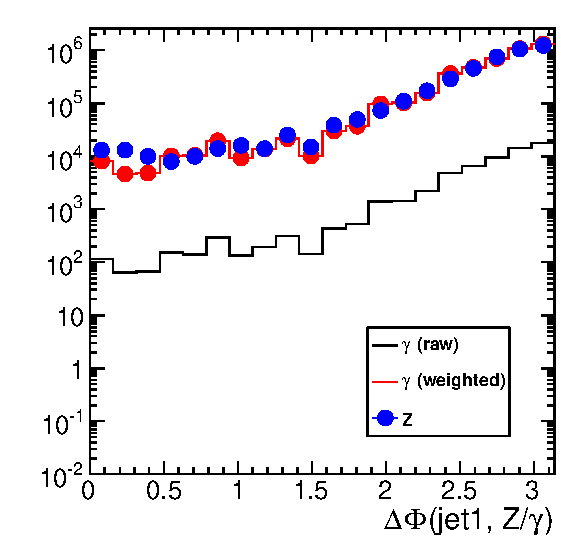
\includegraphics[width=0.3\textwidth]{figures/PhotonJetsClosureTest_0Jet_Dphi.pdf}}
\subfigure[1-Jet]{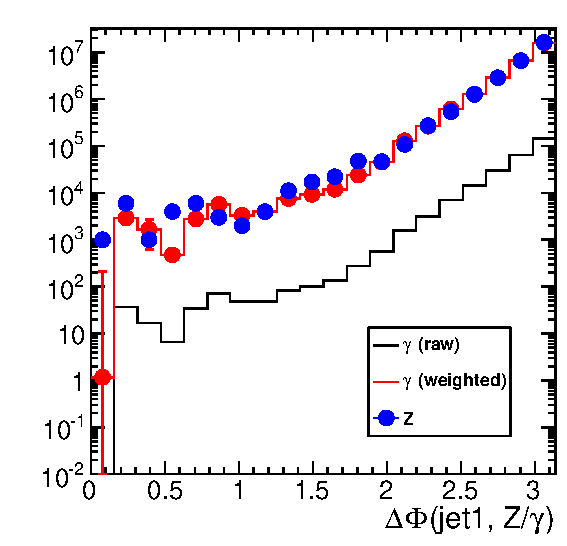
\includegraphics[width=0.3\textwidth]{figures/PhotonJetsClosureTest_1Jet_Dphi.pdf}}
\subfigure[2-Jet]{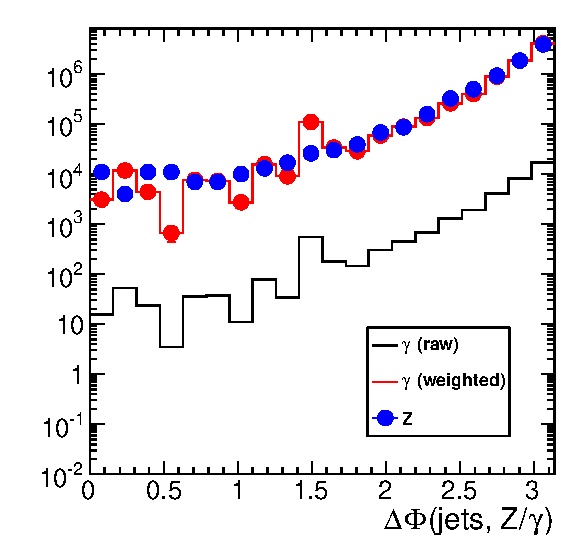
\includegraphics[width=0.3\textwidth]{figures/PhotonJetsClosureTest_2Jet_Dphi.pdf}}
\caption{Comparison of the $\Delta\phi$ between the dilepton system and the leading jet 
(with $p_{T} > 15$ GeV) in the event between the reweighted $\gamma$+jets sample and the 
simulation prediction from the $Z$+jets sample.}
\label{fig:PhotonJetsClosureTest_DPhi}
\end{center}
\end{figure}


Finally, we show the comparison between the predicted transverse mass distribution and the simulation
distribution with no cut on minimum \met in Fig \ref{fig:PhotonJetsClosureTest_MtHZZ_NoMetCut} and 
with a minimum \met cut of greater than $40$GeV in Fig \ref{fig:PhotonJetsClosureTest_MtHZZ_MetPresel}. 
The predicted shape and the simulation shape are again in reasonable agreement. 

\begin{figure}[!htbp]
\begin{center}
\subfigure[0-Jet]{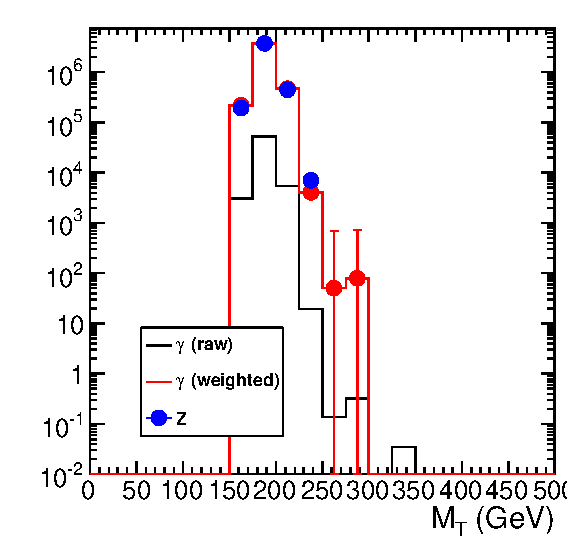
\includegraphics[width=0.3\textwidth]{figures/PhotonJetsClosureTest_0Jet_MtHZZ_NoMetCut.pdf}}
\subfigure[1-Jet]{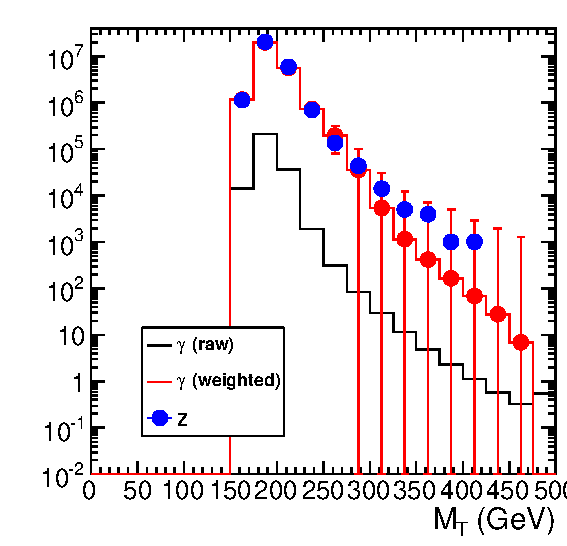
\includegraphics[width=0.3\textwidth]{figures/PhotonJetsClosureTest_1Jet_MtHZZ_NoMetCut.pdf}}
\subfigure[2-Jet]{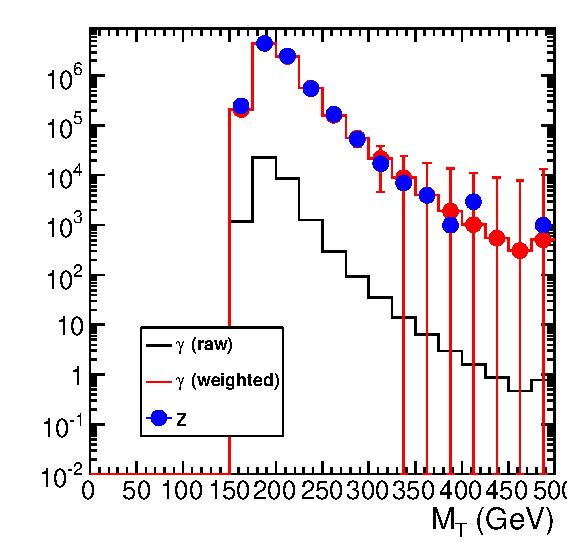
\includegraphics[width=0.3\textwidth]{figures/PhotonJetsClosureTest_2Jet_MtHZZ_NoMetCut.pdf}}
\caption{Comparison of the transverse mass prediction from the reweighted $\gamma$+jets sample 
and the simulation prediction from the $Z$+jets sample, where no \met cut has been applied.}
\label{fig:PhotonJetsClosureTest_MtHZZ_NoMetCut}
\end{center}
\end{figure}

\begin{figure}[!htbp]
\begin{center}
\subfigure[0-Jet]{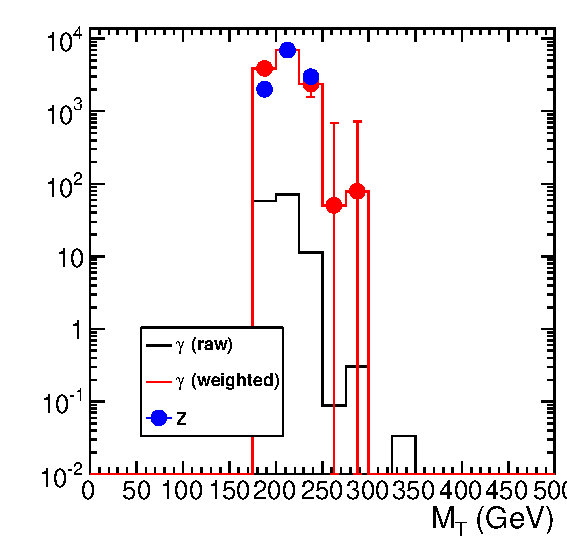
\includegraphics[width=0.3\textwidth]{figures/PhotonJetsClosureTest_0Jet_MtHZZ_MetPresel.pdf}}
\subfigure[1-Jet]{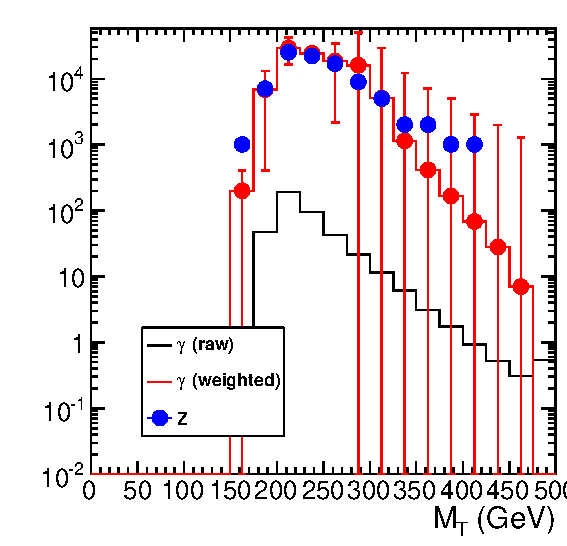
\includegraphics[width=0.3\textwidth]{figures/PhotonJetsClosureTest_1Jet_MtHZZ_MetPresel.pdf}}
\subfigure[2-Jet]{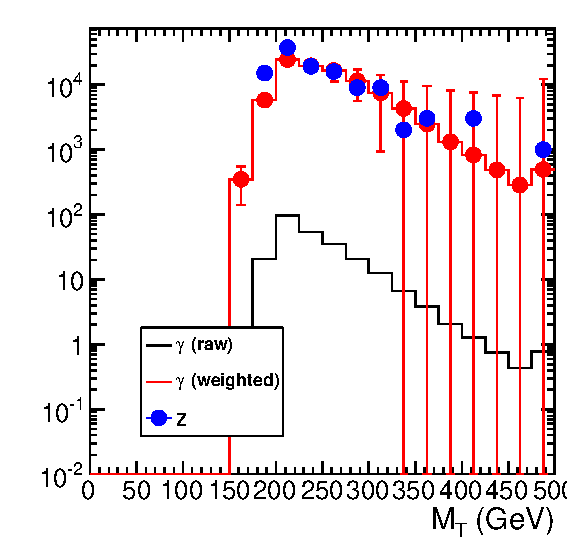
\includegraphics[width=0.3\textwidth]{figures/PhotonJetsClosureTest_2Jet_MtHZZ_MetPresel.pdf}}
\caption{Comparison of the transverse mass prediction from the reweighted $\gamma$+jets sample 
and the simulation prediction from the $Z$+jets sample, where the minimum \met is required to be larger than 
$40$ GeV. }
\label{fig:PhotonJetsClosureTest_MtHZZ_MetPresel}
\end{center}
\end{figure}


%We work on this section more later
%\subsubsection{Systematic Uncertainties}

Based on the degree of overall disagreement in the full range of the minimum \met we assign 
systematic uncertainties of $30\%$ in all the jet bins.


\subsubsection{Data Estimate}

The predictions for the minimum \met and MT are compared with the results obtained in the first $1092\ipb$ 
of Run2011 data in Figures \ref{fig:PhotonJetsDataPreselMinMet} and \ref{fig:PhotonJetsDataPreselMinMet} respectively
This is done sparately for the 0-jet and 1-jet bins. 
Including all of the backgrounds with real \met, we obtain reasonable agreement with data. 

Based on the $\gamma$+jet sample prediction, we obtain the background predictions for the
preselection and all the mass dependent cut-based analyses summarized in Table \ref{tab:DYBkgPrediction}.

\begin{table}[!htbp]
\begin{center}
{\footnotesize
\begin{tabular}{|l|c|c|c|c|}
\hline
Higgs Mass      &  0-jet bin             & 1-jet bin             & 2-jet bin             & Total                \\
\hline
ZZ Preselection &  $16.34\pm0.15\pm4.9$ (stat) & $17.57\pm0.15\pm5.27$(stat)       & $99.10\pm0.24\pm29.73$(stat) & $133.0\pm0.32\pm30.59$(stat) \\ \hline
250             &  $6.73\pm0.11\pm2.00$ (stat)  & $4.76\pm0.03\pm1.43$(stat)       & N/A                          & $11.49\pm0.11\pm2.46$(stat)\\
300             &  $0.51\pm0.05\pm0.15$ (stat)  & $0.33\pm0.01\pm0.01$(stat)       & N/A                          & $0.84\pm0.05\pm0.15$(stat)\\
400             &  $0.00\pm0.00\pm0.00$ (stat)  & $0.87\pm0.07\pm0.26$(stat)       & N/A                          & $0.87\pm0.07\pm0.26$(stat)\\
\hline
\end{tabular}
}
\caption{Summary of $Z$+jets background yields estimated using $\gamma$+jets events in 1092 $\ipb$.}
\label{tab:DYBkgPrediction}
\end{center}
\end{table}

%
% plots in data at the preselection stage 
%

\begin{figure}[!htbp]
\begin{center}
\subfigure[0-Jet]{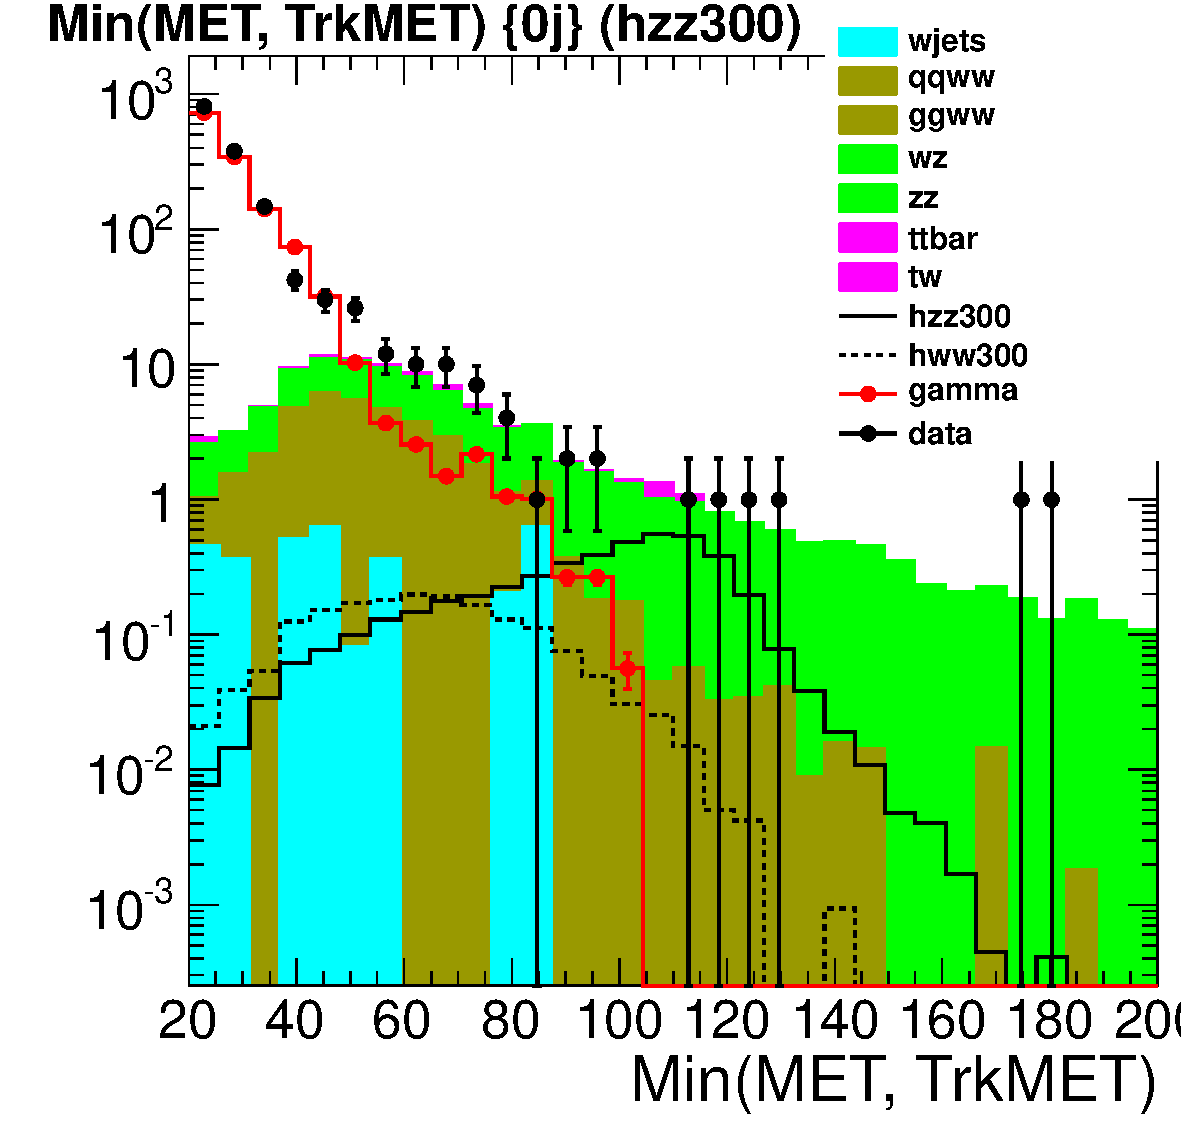
\includegraphics[width=0.45\textwidth]{figures/hzz300_minmet_0j_log.pdf}}
\subfigure[1-Jet]{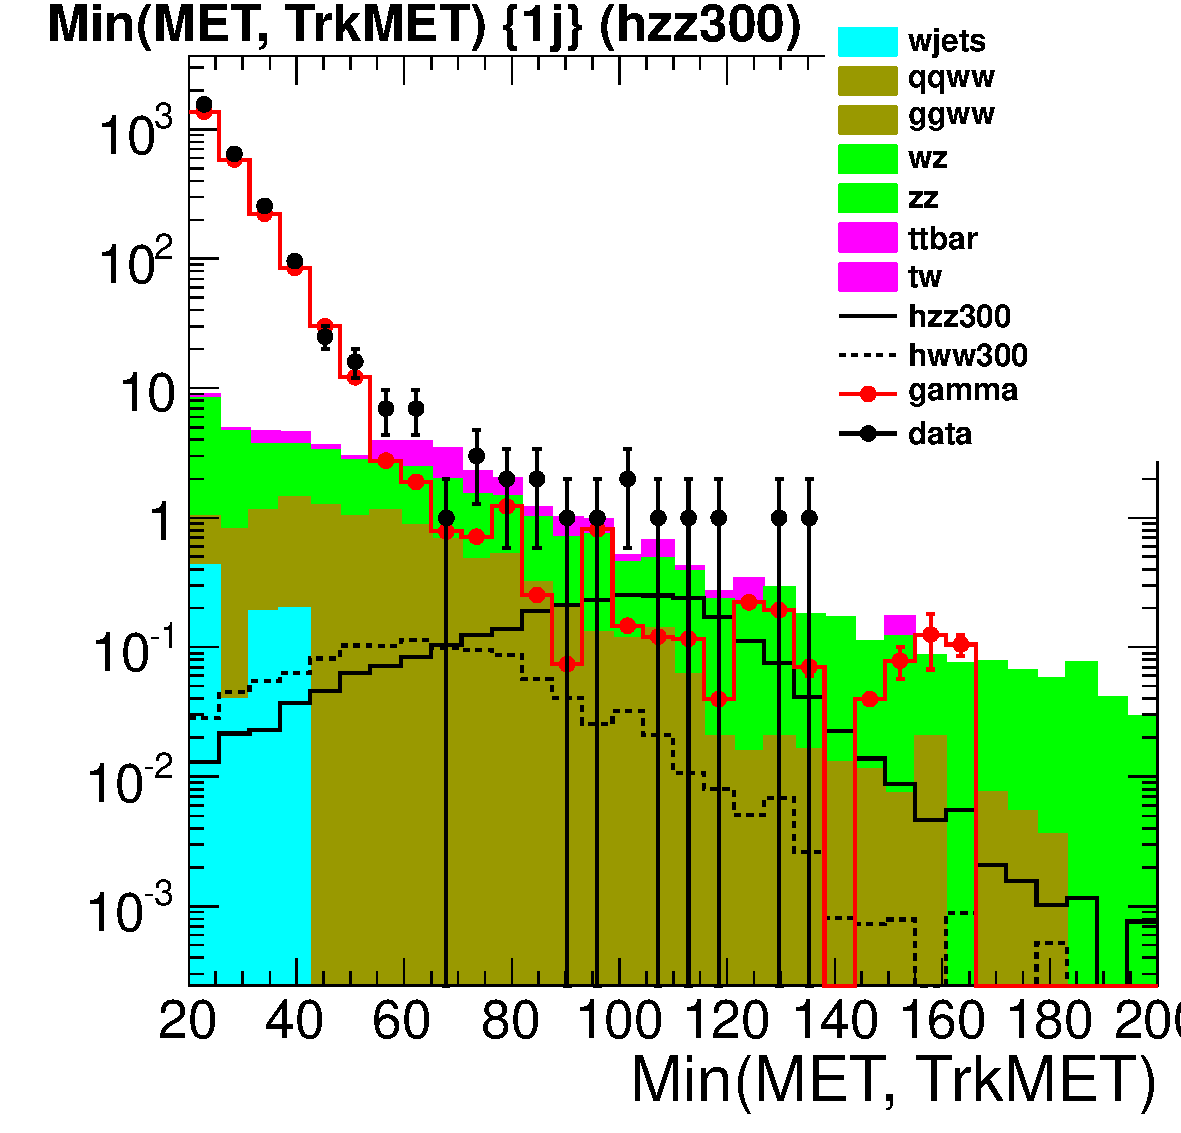
\includegraphics[width=0.45\textwidth]{figures/hzz300_minmet_1j_log.pdf}}
\caption{Comparison of the minimum of the \met and track \met rediction from the reweighted $\gamma$+jets sample
and the dilepton data sample in 1092 $\ipb$. The non Drell-Yan backgrounds are stacked MC scaled from data as appropriate.
The reweighted $\gamma$+jets prediction is not stacked dle FIXME.}
\label{fig:PhotonJetsDataPreselMinMet}
\end{center}
\end{figure}

\begin{figure}[!htbp]
\begin{center}
\subfigure[0-Jet]{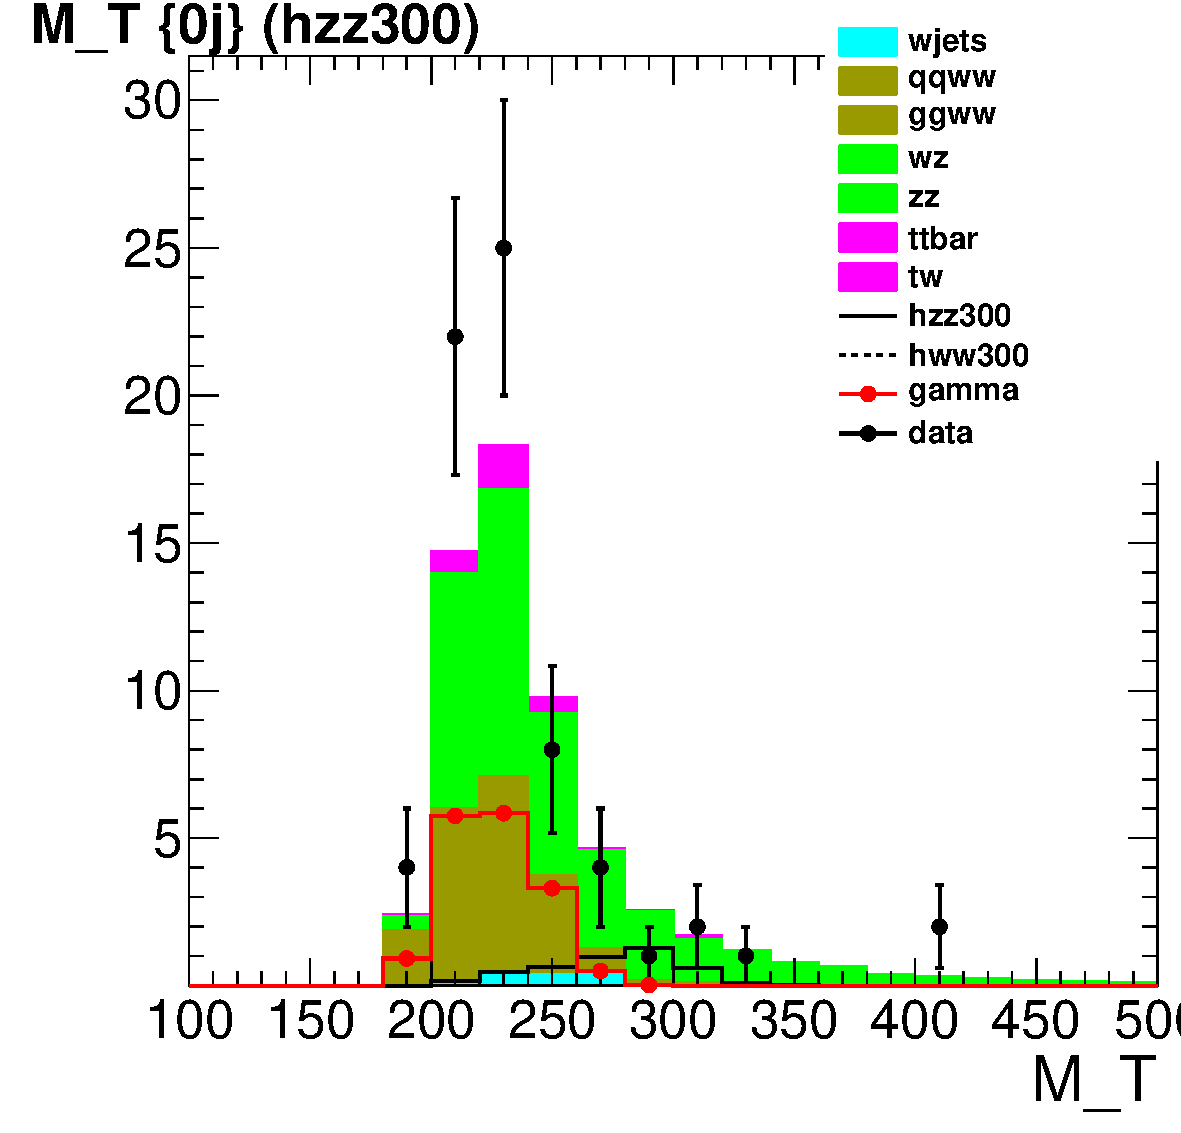
\includegraphics[width=0.45\textwidth]{figures/hzz300_mt_0j.pdf}}
\subfigure[1-Jet]{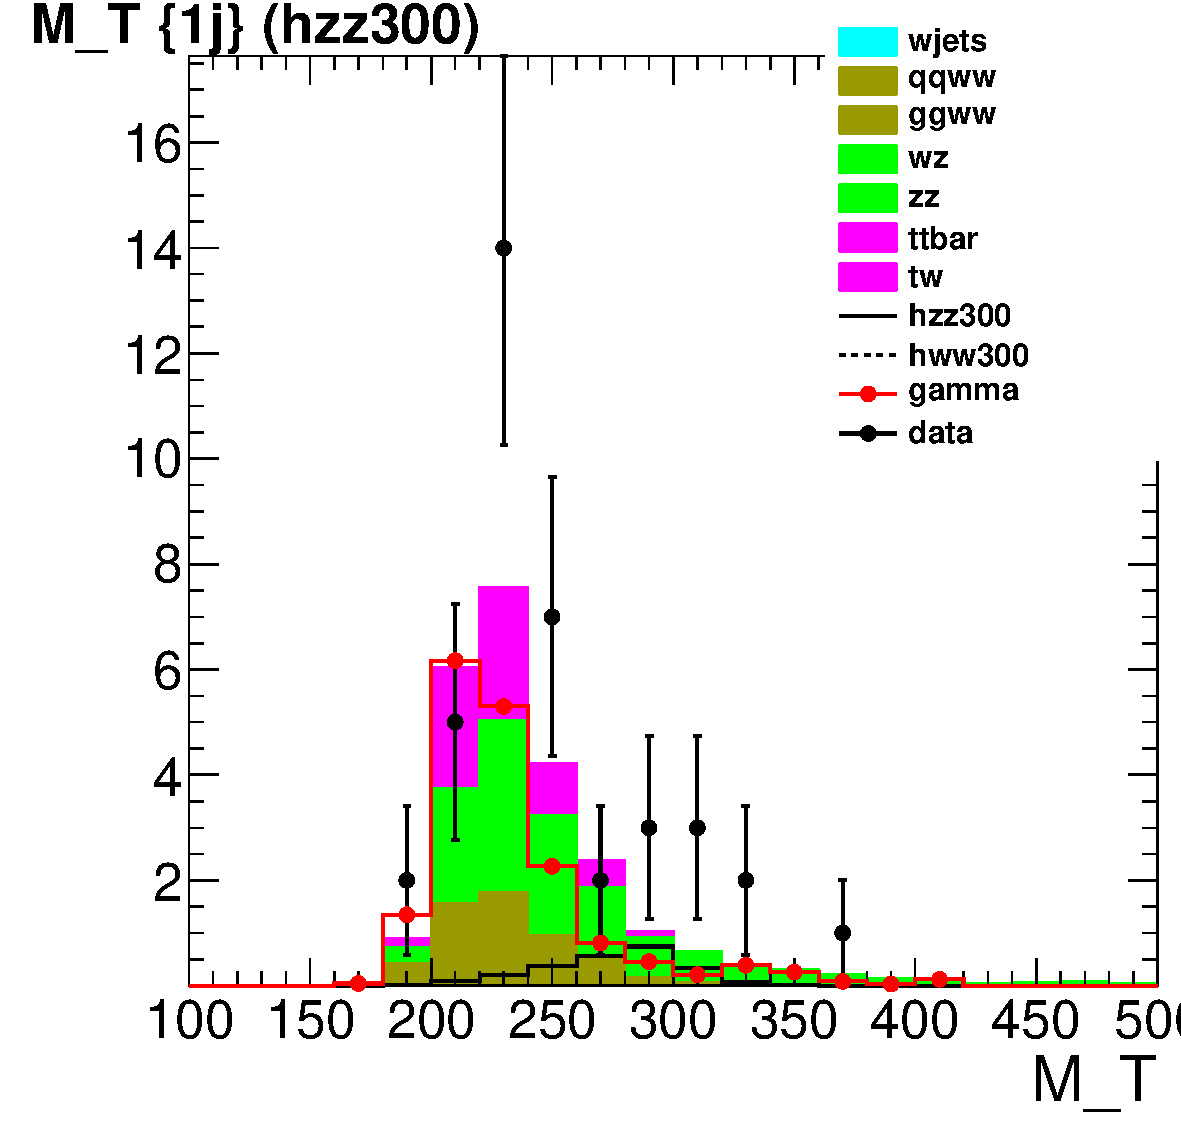
\includegraphics[width=0.45\textwidth]{figures/hzz300_mt_1j.pdf}}
\caption{Comparison of the MT prediction from the reweighted $\gamma$+jets sample
and the dilepton data sample in 1092 $\ipb$ after requiring the minimum of \met and tracker \met to be above 50 GeV. 
The non Drell-Yan backgrounds are stacked MC scaled from data as appropriate.
The reweighted $\gamma$+jets prediction is not stacked dle FIXME.}
\label{fig:PhotonJetsDataPreselMT}
\end{center}
\end{figure}

